\begin{figure}
 \centering  % this centres figure in column
  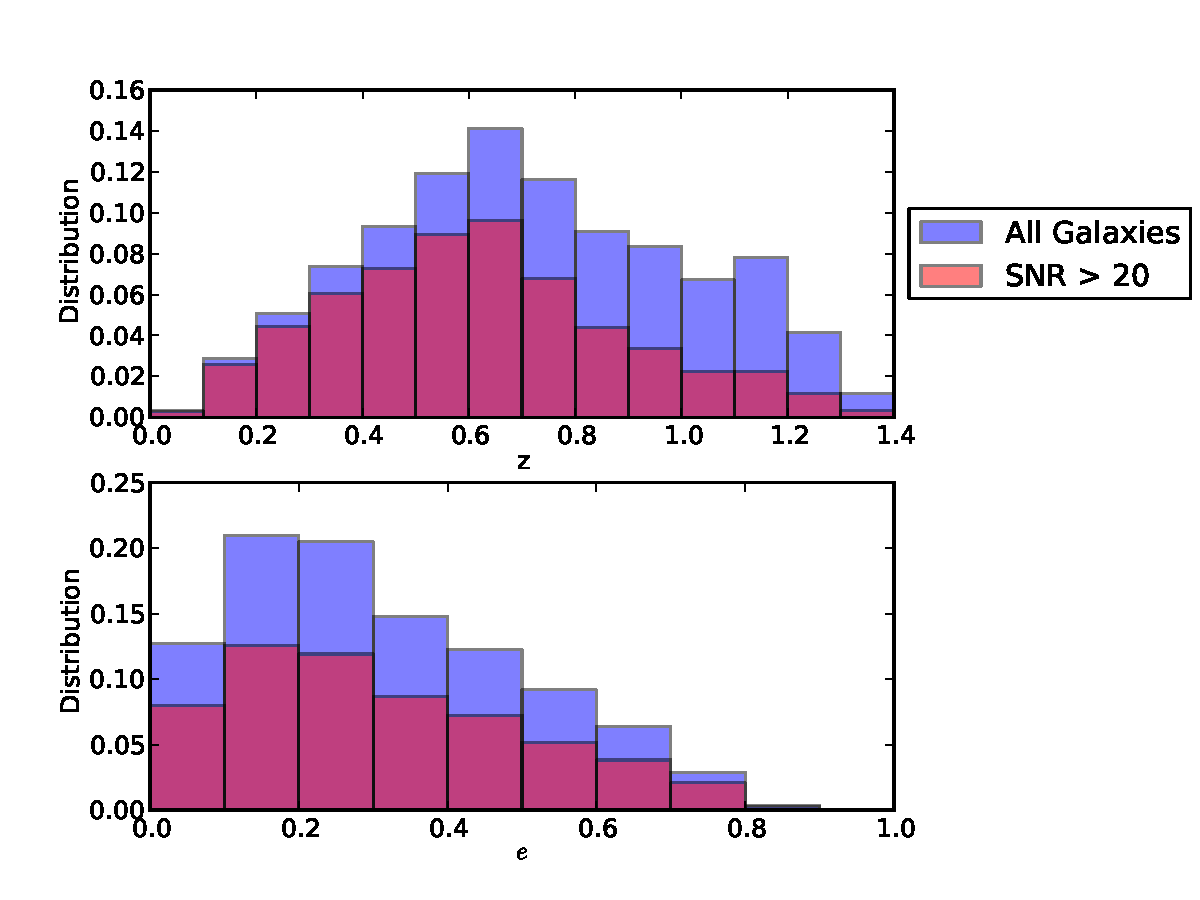
\includegraphics[width=0.45\textwidth]{fig/Out_hist_v2_truth.pdf} 
  \caption{Distributions of various galaxy 
properties in the CSTEP simulation. The top plot shows the
redshift distribution of galaxies as a function of percentage in the simulation. 
The bottom plot shows the distribution of intrinsic ellipticity as a
function of percentage of total objects. The
total number of galaxy objects included is 141559 and is shown in blue, the number of
galaxy obejects with SNR $>$ 20 is 84586 and is shown in magenta.}
\label{fig:Galprop}
\end{figure}
The image simulations used in the CSTEP project were designed to 
replicate the properties of the final co-added data that will be taken by the 
Dark Energy Survey. The Dark Energy survey is an optical survey of
5000 deg$^2$ of the southern sky, that will image around 300 million
galaxies in five filters (g,r,i,z and Y) \citep{Klaus}. To test the DES
data management system and software pipelines developed by the 
science working groups detailed image simulations were created by the 
DES Simulation team \citep{DESsim}. Each simulated image used in CSTEP models the DES focal plane
with 62 CCDs each of which is 2K x 4K pixel (0.27''/pixel). Star and galaxy objects are
rendered by drawing random samples of
photons from the theoretical light profile of the source convolved 
by the PSF. \\
\indent For the CSTEP simulated images, mock galaxy catalogs were
created with the ADDGALS  method that reproduce observed correlations
for galaxies among clustering, luminosities, and colors. 
The parent N-body simulations used by ADDGALS are the ``Carmen'' Las Damas
N-body simulation box (1 Gpc/$H^3$ ) with  $ \Lambda$ cosmology, $\Omega_M
= 0.25, \sigma_8 = 0.8$, at $z< 1.35 $
(\cite{LasDamas}). In each image around $ 140,000 $ galaxy objects are
present. The simulated galaxy images are designed to have similar properties to
the galaxies that DES will observe by combining a mock
catalog with empirical data from the HST/GEMS catalog for galaxies
with magnitude r $ > $ 23 , and from the SDSS for
galaxies with magnitude r $ < $ 23. The distributions of galaxy
properties in the simulation are shown in Figure \ref{fig:Galprop}. 
The galaxy objects are created with Sersic profiles with an
index that ranges from 0.5 to 5.  \\
\indent The CSTEP simulated images contain a constant
PSF which eliminates the technical challenge of determining the best
way to model a varying PSF. For CSTEP there are two
branches in the image simulation sets, those that include a circular
Gaussian PSF and those that include an elliptical Gaussian PSF. 
The elliptical Gaussian PSF has $ \epsilon =
0.03 $. For both the Gaussian and elliptical Gaussian
PSF the simulated images contain a convolution kernel that mimics the
range of isotropic distortion due to the atmosphere that DES will
likely observe. This isotropic distortion simulates seeing conditions,
or atmospheric blurring, of $ 0.7 - 0.9 $ arcsec. 
A summary of the PSF image properties is included in Table \ref{table:tab2}. 
For each PSF there are 8 focal plane images that contain constant
shear for $\gamma = 0.0$ to $\gamma = 0.15$ in both
$\gamma_1$ and $\gamma_2$, as described in Table \ref{table:tab2}.  
\begin{table}
\begin{centering}
\begin{tabular}{ccc}
\hline
PSF Number & Type & Seeing  \\
\hline
1 & circular Gaussian & 0.7 \\
2 & circular Gaussian & 0.8 \\
3 & circular Gaussian & 0.9 \\
4 & elliptical Gaussian & 0.75 \\
5 & elliptical Gaussian & 0.8  \\
6 & elliptical Gaussian & 0.9  \\
\hline
\hline
Shear Number & $ \gamma_1 $ & $ \gamma_2 $  \\
\hline
1 &  0.0 & 0.03 \\
2 &  0.0 & 0.06 \\
3 &  0.0 & 0.09 \\
4 &  0.0 & 0.15 \\
5 &  0.03 & 0.0 \\
6 &  0.06 & 0.0 \\
7 &  0.09 & 0.0 \\
8 &  0.15 & 0.0 \\
\hline
\end{tabular}
\end{centering}
\caption{ Summary of the PSF and shear sets for the CSTEP simulated images. }
\label{table:tab2}
\end{table}
